\documentclass[tikz,border=6pt]{standalone}
\usepackage{amssymb}
\usepackage{amsfonts}
\usepackage{mathrsfs}
\usepackage{amsthm}
\usepackage{amsmath}
\usepackage{xcolor}
\usepackage{hyperref}
\usepackage{libertinus}
\usepackage{dsfont}
\usepackage{bm}
\usepackage{enumitem}
\usepackage{caption}
\usepackage{subcaption}
\usepackage{tikz}
\usepackage{quiver}

\newcommand{\R}{\mathbb{R}}
\newcommand{\C}{\mathbb{C}}
\newcommand{\N}{\mathbb{N}}
\newcommand{\Z}{\mathbb{Z}}
\newcommand{\Q}{\mathbb{Q}}

\newcommand{\id}{\operatorname{id}}

% differentials and derivatives
\renewcommand{\d}{\mathrm{d}}
\newcommand{\dd}{\,\d}
\newcommand{\pddf}[2]{\frac{\partial#1}{\partial#2}}
\newcommand{\ddt}{\frac{\d }{\d t}}
\newcommand{\ddtz}{\left.\ddt\right|_{t=0}}

\begin{document}
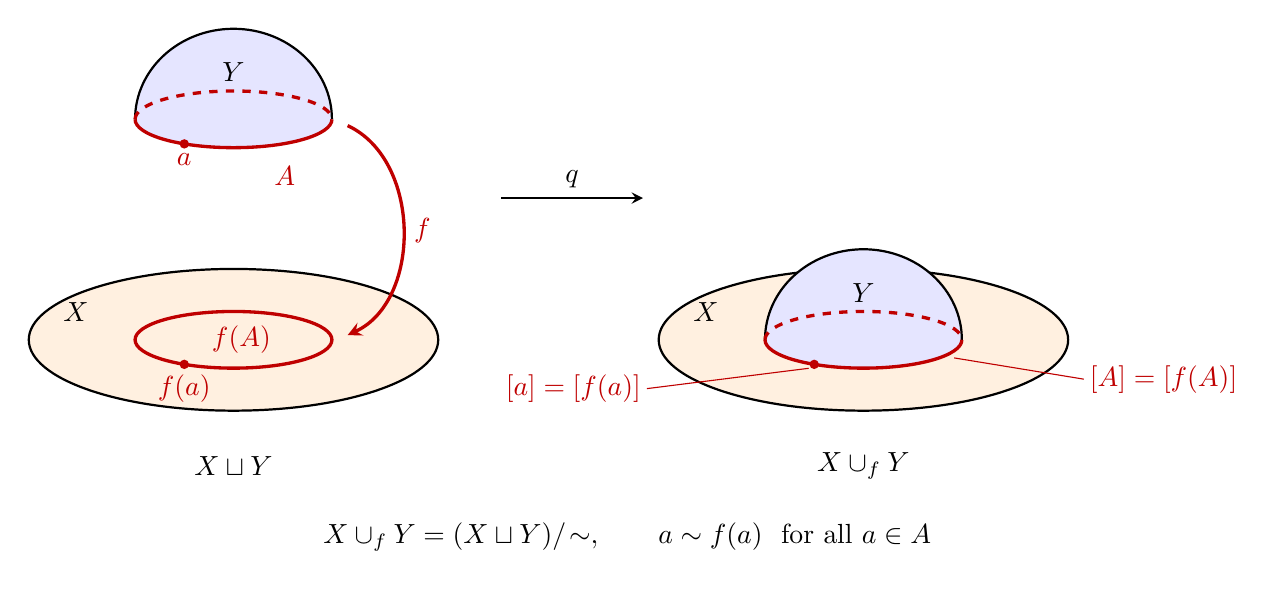
\begin{tikzpicture}[
    >=stealth,
    surface/.style={thick},
    glue/.style={red!75!black, very thick},
]

    \def\capr{1.25}      % radius of the cap Y, i.e. of the circle A
    \def\caph{1.15}      % height of the cap Y
    \def\persp{0.36}     % half-height of a circle of radius \capr in perspective
    \def\brimr{2.6}      % radius of the disk X
    \def\brimp{0.9}      % half-height of the disk X in perspective
    \def\ang{-120}       % the marked point a sits at this angle on A

    % =============================================================
    % Left: the disjoint union X \sqcup Y, together with f : A \to X
    % =============================================================

    % Y is a cap; its boundary circle is the closed subspace A
    \begin{scope}[shift={(0,2.8)}]
        \fill[blue!10]
            (-\capr,0)
            arc[start angle=180, end angle=0, x radius=\capr, y radius=\caph]
            arc[start angle=0, end angle=-180, x radius=\capr, y radius=\persp]
            -- cycle;
        \draw[surface] (-\capr,0)
            arc[start angle=180, end angle=0, x radius=\capr, y radius=\caph];
        \draw[glue, dashed] (-\capr,0)
            arc[start angle=180, end angle=0, x radius=\capr, y radius=\persp];
        \draw[glue] (\capr,0)
            arc[start angle=0, end angle=-180, x radius=\capr, y radius=\persp];

        \node at (0,0.6) {$Y$};
        \node[glue] at (0.65,-0.72) {$A$};
        \fill[glue] ({\capr*cos(\ang)},{\persp*sin(\ang)}) circle (1.7pt)
            node[anchor=north, inner sep=3pt] {$a$};
    \end{scope}

    % X is a disk; the image f(A) is a circle inside it
    \fill[orange!12] (0,0) ellipse ({\brimr} and {\brimp});
    \draw[surface] (0,0) ellipse ({\brimr} and {\brimp});
    \draw[glue] (0,0) ellipse ({\capr} and {\persp});
    \node at (-2,0.35) {$X$};
    \node[glue] at (0.1,0) {$f(A)$};
    \fill[glue] ({\capr*cos(\ang)},{\persp*sin(\ang)}) circle (1.7pt)
        node[anchor=north, inner sep=3pt] {$f(a)$};

    % f maps A onto f(A)
    \draw[->, glue] (1.45,2.72)
        to[out=-25, in=25] node[pos=0.5, right] {$f$} (1.45,0.06);

    \node at (0,-1.6) {$X\sqcup Y$};

    % =============================================================
    % Right: the attaching space, a hat with brim X and crown Y
    % =============================================================
    \begin{scope}[shift={(8,0)}]
        \fill[orange!12] (0,0) ellipse ({\brimr} and {\brimp});
        \draw[surface] (0,0) ellipse ({\brimr} and {\brimp});

        % The crown is opaque: it hides the far side of the brim
        \fill[blue!10]
            (-\capr,0)
            arc[start angle=180, end angle=0, x radius=\capr, y radius=\caph]
            arc[start angle=0, end angle=-180, x radius=\capr, y radius=\persp]
            -- cycle;
        \draw[surface] (-\capr,0)
            arc[start angle=180, end angle=0, x radius=\capr, y radius=\caph];
        \draw[glue, dashed] (-\capr,0)
            arc[start angle=180, end angle=0, x radius=\capr, y radius=\persp];
        \draw[glue] (\capr,0)
            arc[start angle=0, end angle=-180, x radius=\capr, y radius=\persp];

        \node at (0,0.6) {$Y$};
        \node at (-2,0.35) {$X$};

        \fill[glue] ({\capr*cos(\ang)},{\persp*sin(\ang)}) circle (1.7pt);
        \draw[glue, thin] ({\capr*cos(\ang)-0.07},{\persp*sin(\ang)-0.05})
            -- (-2.75,-0.62)
            node[anchor=east, inner sep=2pt] {$[a]=[f(a)]$};
        \draw[glue, thin] ({\capr*cos(-30)+0.07},{\persp*sin(-30)-0.05})
            -- (2.8,-0.5)
            node[anchor=west, inner sep=2pt] {$[A]=[f(A)]$};

        \node at (0,-1.6) {$X\cup_{f}Y$};
    \end{scope}

    % The quotient map
    \draw[->, thick] (3.4,1.8) -- node[above] {$q$} (5.2,1.8);

    \node[anchor=north] at (5,-2.2)
        {$X\cup_{f}Y=(X\sqcup Y)/\!\sim,
          \qquad a\sim f(a)\ \text{ for all } a\in A$};

\end{tikzpicture}
\end{document}
